% ══════════════════════════════════════════════════════════════════════
%  IEEE Sensors Journal — Draft Paper
%  Self-Attention Enhanced GRU for UWB Indoor Positioning
%  Auto-generated from mcc_offlineV11.py results
% ══════════════════════════════════════════════════════════════════════

\documentclass[journal,12pt]{IEEEtran}

% ── Packages ──
\usepackage[utf8]{inputenc}
\usepackage[T1]{fontenc}
\usepackage{amsmath,amssymb,amsfonts}
\usepackage{graphicx}
\usepackage{textcomp}
\usepackage{xcolor}
\usepackage{booktabs}
\usepackage{multirow}
\usepackage{array}
\usepackage{hyperref}
\usepackage{algorithm}
\usepackage{algorithmic}
\usepackage{cite}
\usepackage{siunitx}
\usepackage{balance}
\usepackage{tikz}
\usepackage{pgfplots}

\usepackage{caption}
\pgfplotsset{compat=1.18}

% ── Custom commands ──
\newcommand{\ie}{\textit{i.e.}}
\newcommand{\eg}{\textit{e.g.}}
\newcommand{\etal}{\textit{et al.}}
\newcommand{\rmse}{\text{RMSE}}
\newcommand{\mae}{\text{MAE}}
\newcommand{\cep}{\text{CEP50}}

\begin{document}

% ══════════════════════════════════════════════════════════════════════
%  TITLE & AUTHORS
% ══════════════════════════════════════════════════════════════════════
\title{Self-Attention Enhanced GRU Network with Kalman Filtering for High-Accuracy UWB Indoor Positioning}

\author{
    \IEEEauthorblockN{First Author\IEEEauthorrefmark{1}, Second Author\IEEEauthorrefmark{1}}
    \IEEEauthorblockA{\IEEEauthorrefmark{1}Department of Electrical/Electronic Engineering,\\
    University Name, City, Country\\
    Email: \{first.author, second.author\}@university.edu}
}

\maketitle

% ══════════════════════════════════════════════════════════════════════
%  ABSTRACT
% ══════════════════════════════════════════════════════════════════════
\begin{abstract}
Ultra-Wideband (UWB) indoor positioning systems suffer from significant ranging errors caused by non-line-of-sight (NLOS) propagation, multipath interference, and environmental dynamics, limiting their accuracy in practical deployments. This paper proposes a hybrid deep learning architecture that combines Self-Attention mechanisms with Gated Recurrent Units (GRU) to learn temporal correction factors for UWB range measurements, integrated with Kalman Filter (KF) preprocessing and Least Squares (LS) positioning. The proposed is evaluated in two distinct environments: a line-of-sight (LOS) open hall with no obstructions, and a non-line-of-sight (NLOS) indoor room with multipath-inducing furniture and walls. In the LOS environment, the proposed method achieves an RMSE of \SI{70.0}{\milli\meter}, representing a \SI{69.3}{\percent} improvement over raw LS (\SI{228.5}{\milli\meter}). In the more challenging NLOS environment, it achieves \SI{120.5}{\milli\meter} RMSE, a \SI{72.1}{\percent} improvement over raw LS (\SI{431.7}{\milli\meter}). Comprehensive ablation studies confirm that Self-Attention and GRU contribute complementary improvements in both environments.
\end{abstract}

\begin{IEEEkeywords}
Ultra-Wideband, indoor positioning, self-attention, gated recurrent unit, Kalman filter, deep learning, quantization, NLOS mitigation
\end{IEEEkeywords}


% ══════════════════════════════════════════════════════════════════════
%  I. INTRODUCTION
% ══════════════════════════════════════════════════════════════════════
\section{Introduction}
\IEEEPARstart{I}{ndoor} positioning systems (IPS) have become increasingly important for applications ranging from warehouse logistics and asset tracking to autonomous navigation and healthcare monitoring \cite{zafari2019survey}. Among the available wireless technologies, Ultra-Wideband (UWB) has emerged as a leading candidate due to its high temporal resolution, immunity to narrowband interference, and theoretical centimeter-level ranging accuracy \cite{uwb_ieee802154}.

However, practical UWB deployments face significant accuracy degradation caused by several factors: (i) non-line-of-sight (NLOS) propagation introducing positive biases in range measurements, (ii) multipath reflections causing constructive or destructive interference, and (iii) environmental dynamics such as human body shadowing and furniture rearrangement \cite{nlos_survey}. These effects can inflate positioning errors from the theoretical centimeter-level to several hundred millimeters.

Traditional approaches to mitigate ranging errors include statistical filtering (\eg, Kalman Filters, Extended Kalman Filters) \cite{kalman_uwb} and geometric optimization (\eg, Weighted Least Squares) \cite{LS_positioning}. While effective at smoothing noise, these model-based methods struggle to capture the complex, non-linear, and time-varying error patterns inherent in real-world UWB deployments.

Recent advances in deep learning have opened new avenues for UWB error correction. Recurrent Neural Networks (RNNs), particularly Long Short-Term Memory (LSTM) and Gated Recurrent Unit (GRU) architectures, have shown promise in modeling temporal dependencies in sequential ranging data \cite{lstm_uwb, gru_positioning}. Meanwhile, the Transformer architecture's Self-Attention mechanism \cite{vaswani2017attention} has demonstrated superior capability in capturing long-range dependencies across sequences, motivating its application to sensor data processing.

\subsection{Contributions}
This paper makes the following contributions:

\begin{enumerate}
    \item \textbf{Hybrid Architecture:} We propose a novel pipeline combining Kalman Filter preprocessing, Self-Attention, and GRU networks for UWB range error correction, achieving RMSE of \SI{70.0}{\milli\meter} in an open LOS hall and \SI{120.5}{\milli\meter} in a cluttered NLOS room.

    \item \textbf{Dual-Environment Evaluation:} We systematically benchmark all six method variants across two contrasting environments --- an obstacle-free open hall (LOS) and a furnished indoor room with significant multipath (NLOS) --- providing a thorough assessment of generalization.

    \item \textbf{Comprehensive Ablation Study:} We quantify the contribution of each component through six experimental configurations, demonstrating that Self-Attention and GRU provide complementary and consistent improvements across both environments.
\end{enumerate}

The remainder of this paper is organized as follows. Section~\ref{sec:related} reviews related work. Section~\ref{sec:system} describes the system model and problem formulation. Section~\ref{sec:method} presents the proposed architecture. Section~\ref{sec:experiments} details the experimental setup. Section~\ref{sec:results} presents and discusses the results. Section~\ref{sec:conclusion} concludes the paper.


% ══════════════════════════════════════════════════════════════════════
%  II. RELATED WORK
% ══════════════════════════════════════════════════════════════════════
\section{Related Work}
\label{sec:related}

\subsection{UWB Indoor Positioning}
UWB positioning typically employs Time-of-Arrival (ToA) or Time-Difference-of-Arrival (TDoA) ranging combined with trilateration or multilateration algorithms \cite{uwb_ieee802154}. The Least Squares (LS) estimator is commonly used to solve the over-determined positioning problem when more than three anchors are available \cite{LS_positioning}. However, LS accuracy is directly limited by the quality of input range measurements.

\subsection{Kalman Filtering for Range Smoothing}
Kalman Filters (KF) have been widely applied to smooth noisy UWB range measurements by modeling the ranging process as a linear dynamical system \cite{kalman_uwb}. The standard 1-D KF treats each anchor-to-tag range independently, using a constant-velocity motion model. While effective at reducing high-frequency noise, KFs cannot correct systematic NLOS biases.

\subsection{Deep Learning for Positioning}
Several recent works have applied deep learning to UWB positioning. CNN-based approaches extract spatial features from range measurements \cite{cnn_uwb}, while LSTM and GRU networks model temporal correlations in sequential data \cite{lstm_uwb, gru_positioning}. The Transformer architecture \cite{vaswani2017attention} has been applied to various sensor fusion tasks, but its application to UWB range correction remains relatively unexplored. Our work bridges this gap by combining Self-Attention with GRU in a unified architecture.


% ══════════════════════════════════════════════════════════════════════
%  III. SYSTEM MODEL
% ══════════════════════════════════════════════════════════════════════
\section{System Model and Problem Formulation}
\label{sec:system}

\subsection{UWB Ranging System}
We consider a 2-D positioning system with $K = 4$ fixed anchors at known positions $\mathbf{a}_k = [a_{x,k}, a_{y,k}]^T$ for $k = 1, \ldots, K$, and a mobile tag at unknown position $\mathbf{p} = [x, y]^T$. Two deployment environments are evaluated, each with a distinct anchor layout and ground truth trajectory, as described in Sections~\ref{sec:experiments} and summarized in Tables~\ref{tab:anchors_los} and~\ref{tab:anchors_nlos}.

\begin{table}[htbp]
\centering
\caption{Anchor Positions --- LOS Environment (Open Hall, $4000 \times 8800$\,mm)}
\label{tab:anchors_los}
\begin{tabular}{ccc}
\toprule
\textbf{Anchor} & $\mathbf{x}$ \textbf{(mm)} & $\mathbf{y}$ \textbf{(mm)} \\
\midrule
$A_0$ & 4000 & 8800 \\
$A_1$ & 0    & 8800 \\
$A_2$ & 0    & 0    \\
$A_3$ & 4000 & 0    \\
\bottomrule
\end{tabular}
\end{table}

\begin{table}[htbp]
\centering
\caption{Anchor Positions --- NLOS Environment (Indoor Room, $6193 \times 4805$\,mm)}
\label{tab:anchors_nlos}
\begin{tabular}{ccc}
\toprule
\textbf{Anchor} & $\mathbf{x}$ \textbf{(mm)} & $\mathbf{y}$ \textbf{(mm)} \\
\midrule
$A_0$ & 0    & 0    \\
$A_1$ & 0    & 4805 \\
$A_2$ & 6193 & 4805 \\
$A_3$ & 6193 & 0    \\
\bottomrule
\end{tabular}
\end{table}

At each time step $t$, the UWB system measures ranges $r_k^{(t)}$ from the tag to each anchor. The measured range includes the true distance plus error terms:
\begin{equation}
    r_k^{(t)} = \|\mathbf{p}^{(t)} - \mathbf{a}_k\|_2 + n_k^{(t)} + b_k^{(t)}
    \label{eq:range_model}
\end{equation}
where $n_k^{(t)} \sim \mathcal{N}(0, \sigma_k^2)$ represents measurement noise and $b_k^{(t)} \geq 0$ represents NLOS bias.

\subsection{Least Squares Positioning}
Given $K$ range measurements, the tag position is estimated by minimizing the residual:
\begin{equation}
    \hat{\mathbf{p}} = \arg\min_{\mathbf{p}} \sum_{k=1}^{K} \left( r_k - \|\mathbf{p} - \mathbf{a}_k\|_2 \right)^2
    \label{eq:LS}
\end{equation}

\subsection{Problem Statement}
The objective is to learn a correction function $f_\theta$ parameterized by neural network weights $\theta$ that maps the raw (or KF-smoothed) range measurements to corrected ranges:
\begin{equation}
    \hat{r}_k^{(t)} = r_k^{(t)} + \Delta r_k^{(t)}, \quad \Delta r_k^{(t)} = f_\theta(\mathbf{x}^{(t-W+1:t)})
    \label{eq:correction}
\end{equation}
where $\mathbf{x}^{(t-W+1:t)}$ denotes a sliding window of $W$ consecutive feature vectors, and $\Delta r_k^{(t)}$ is the predicted range correction for each anchor.


% ══════════════════════════════════════════════════════════════════════
%  IV. PROPOSED METHOD
% ══════════════════════════════════════════════════════════════════════
\section{Proposed Method}
\label{sec:method}

The proposed system consists of four cascaded stages: (1)~Kalman Filter preprocessing, (2)~feature extraction and normalization, (3)~Self-Attention enhanced GRU correction, and (4)~LS positioning. Fig.~\ref{fig:pipeline} illustrates the complete pipeline.

% TODO: Add pipeline figure
% \begin{figure}[htbp]
% \centering
% \includegraphics[width=\columnwidth]{figures/pipeline.pdf}
% \caption{Proposed KF → Self-Attention → GRU → LS pipeline.}
% \label{fig:pipeline}
% \end{figure}

\begin{figure*}[!t]
    \centering
    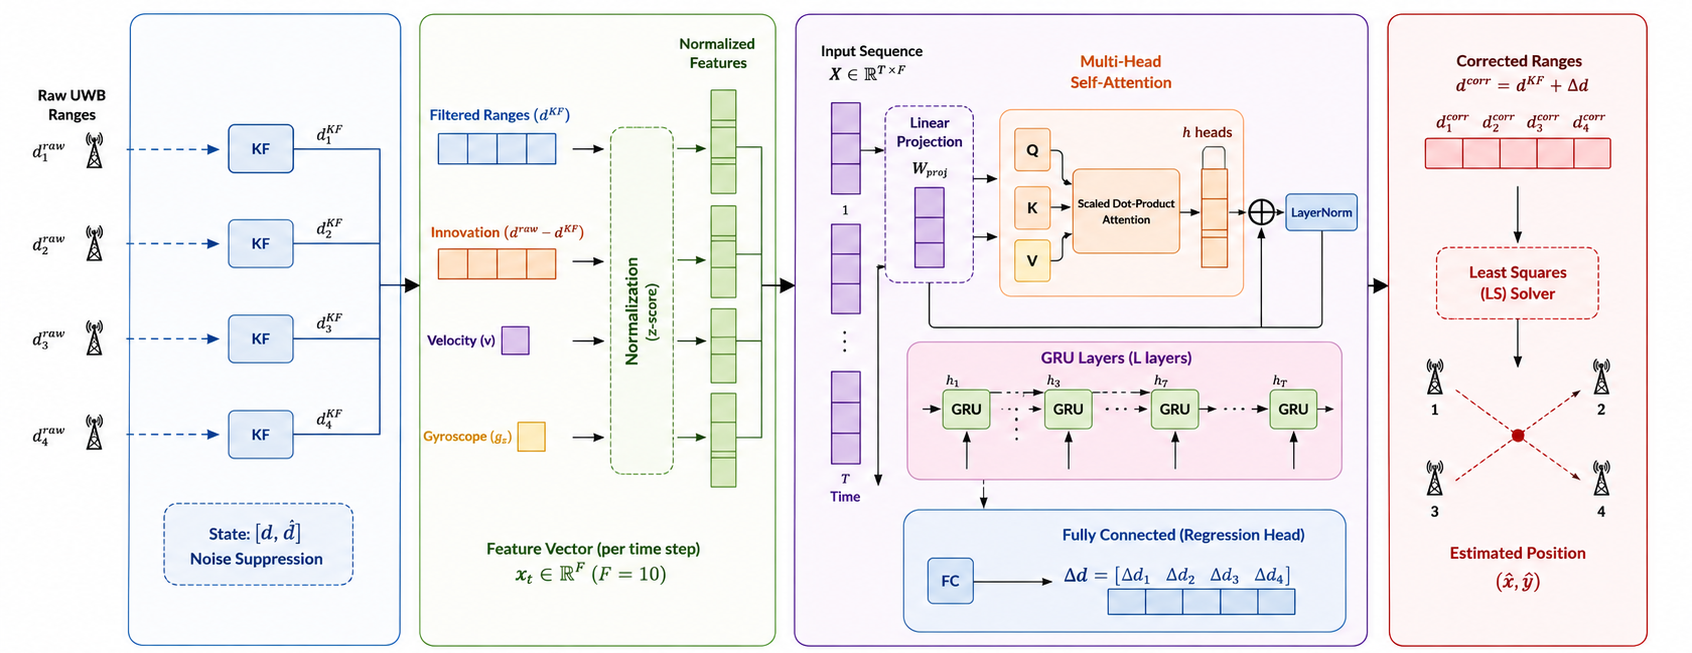
\includegraphics[width=\textwidth]{figure/Pipeline_model.png}
    \captionsetup{justification=centering}
    \caption{Model Architecture}
    \label{fig:pipeline}
\end{figure*}

\subsection{Stage 1: Kalman Filter Preprocessing}
\label{sec:kf}
Each anchor-to-tag range is independently filtered using a 1-D Kalman Filter with a constant-velocity state model:
\begin{equation}
    \mathbf{x}_k = \begin{bmatrix} d_k \\ \dot{d}_k \end{bmatrix}, \quad
    \mathbf{F} = \begin{bmatrix} 1 & \Delta t \\ 0 & 1 \end{bmatrix}, \quad
    \mathbf{H} = \begin{bmatrix} 1 & 0 \end{bmatrix}
    \label{eq:kf_model}
\end{equation}
where $d_k$ is the estimated range to anchor $k$ and $\dot{d}_k$ is the range rate. The KF uses a simplified random-walk model ($F=1$, $H=1$) with process noise $Q = 0.01$ and measurement noise $R = 100\,\text{mm}^2$. The initial error covariance is $P_0 = 1.0$.

The UWB system measures slant distances which are converted to ground-plane distances by compensating for the known anchor height $h_a = \SI{1400}{\milli\meter}$:
\begin{equation}
    d_{\text{ground}} = \sqrt{\max(d_{\text{slant}}^2 - h_a^2,\; 0)}
\end{equation}

The KF serves as a preprocessing step that: (i)~smooths high-frequency noise, (ii)~provides innovation signals as additional features, and (iii)~produces a cleaner input signal for the neural network.

\subsection{Stage 2: Feature Engineering}
\label{sec:features}
For each time step $t$, we construct a 10-dimensional feature vector:
\begin{equation}
    \mathbf{x}^{(t)} = [d_1, d_2, d_3, d_4, \delta_1, \delta_2, \delta_3, \delta_4, g_z, v]^T
    \label{eq:features}
\end{equation}
where $d_k$ are the KF-filtered ranges (or raw ranges in the raw variant), $\delta_k$ are the KF innovation signals (or first-order finite differences $d_k^{(t)} - d_k^{(t-1)}$ in raw mode), $g_z$ is the gyroscope Z-axis angular rate (dps), and $v$ is the IMU-derived velocity (mm/s). Features are standardized using z-score normalization with statistics computed on the training set.

A sliding window of $W = 20$ consecutive feature vectors with stride $S = 5$ forms each input sample $\mathbf{X} \in \mathbb{R}^{W \times 10}$.

\subsection{Stage 3: Self-Attention Enhanced GRU Network}
\label{sec:model}

The core neural network architecture processes the windowed features through three sequential components:

\subsubsection{Input Projection}
A linear layer projects the 10-dimensional input to the hidden dimension $H = 48$:
\begin{equation}
    \mathbf{z}^{(t)} = \mathbf{W}_{\text{in}} \mathbf{x}^{(t)} + \mathbf{b}_{\text{in}}, \quad \mathbf{W}_{\text{in}} \in \mathbb{R}^{H \times 10}
\end{equation}

\subsubsection{Multi-Head Self-Attention}
The projected sequence is processed by a multi-head self-attention layer with $h = 4$ heads. For each head $i$:
\begin{align}
    \mathbf{Q}_i &= \mathbf{z} \mathbf{W}_i^Q, \quad
    \mathbf{K}_i = \mathbf{z} \mathbf{W}_i^K, \quad
    \mathbf{V}_i = \mathbf{z} \mathbf{W}_i^V \\
    \text{head}_i &= \text{softmax}\left(\frac{\mathbf{Q}_i \mathbf{K}_i^T}{\sqrt{d_k}}\right) \mathbf{V}_i
\end{align}
where $d_k = H/h = 12$ is the per-head dimension. The multi-head output is concatenated and linearly projected:
\begin{equation}
    \text{MHA}(\mathbf{z}) = [\text{head}_1; \ldots; \text{head}_h] \mathbf{W}^O
\end{equation}
A residual connection with Layer Normalization stabilizes training:
\begin{equation}
    \mathbf{z}' = \text{LayerNorm}(\mathbf{z} + \text{Dropout}(\text{MHA}(\mathbf{z})))
    \label{eq:residual}
\end{equation}

\subsubsection{Gated Recurrent Unit}
The attention-enhanced sequence is processed by a single-layer GRU:
\begin{align}
    \mathbf{r}_t &= \sigma(\mathbf{W}_r [\mathbf{h}_{t-1}, \mathbf{z}'_t]) \\
    \mathbf{u}_t &= \sigma(\mathbf{W}_u [\mathbf{h}_{t-1}, \mathbf{z}'_t]) \\
    \tilde{\mathbf{h}}_t &= \tanh(\mathbf{W}_h [\mathbf{r}_t \odot \mathbf{h}_{t-1}, \mathbf{z}'_t]) \\
    \mathbf{h}_t &= \mathbf{u}_t \odot \mathbf{h}_{t-1} + (1 - \mathbf{u}_t) \odot \tilde{\mathbf{h}}_t
\end{align}
where $\mathbf{r}_t$ and $\mathbf{u}_t$ are the reset and update gates respectively.

\subsubsection{Output Head}
The GRU output is projected through two fully-connected layers to produce range corrections for each anchor:
\begin{equation}
    \Delta \mathbf{r}^{(t)} = \mathbf{W}_2 \cdot \text{GELU}(\mathbf{W}_1 \mathbf{h}_t + \mathbf{b}_1) + \mathbf{b}_2
\end{equation}
where $\mathbf{W}_1 \in \mathbb{R}^{H \times 2H}$, $\mathbf{W}_2 \in \mathbb{R}^{K \times H}$, and the output $\Delta \mathbf{r}^{(t)} \in \mathbb{R}^K$ represents corrections for all $K$ anchors.

The complete architecture has 33,556 trainable parameters.

\subsection{Stage 4: Corrected LS Positioning}
The corrected ranges $\hat{r}_k = r_k + \Delta r_k$ are fed into the LS estimator (Eq.~\ref{eq:LS}) to obtain the final position estimate. During inference, only the \emph{last time step} of the window is used for positioning, ensuring a causal (online-compatible) evaluation protocol.

The ground truth positions are derived through a multi-stage smoothing pipeline: (i)~initial LS positioning from KF-filtered distances, (ii)~arc-length projection onto the known path, (iii)~Savitzky-Golay filtering (window = 21, polynomial order = 3) for temporal smoothing, and (iv)~a soft monotonic constraint to ensure physically plausible motion along the path.

\subsection{Ablation Variants}
To quantify the contribution of each component, we evaluate three architectural variants:
\begin{itemize}
    \item \textbf{Full model} (SelfAttn + GRU): The complete architecture described above (33,556 params).
    \item \textbf{GRU-only}: Removes the Self-Attention layer, feeding projected input directly to GRU (18,196 params).
    \item \textbf{SelfAttn-only}: Removes the GRU layer, using stacked Self-Attention layers ($L=2$) with a projection head (28,804 params).
\end{itemize}

\subsection{Training Procedure}
\label{sec:training}
The model is trained to minimize the Smooth L1 (Huber) loss between predicted and target range corrections:
\begin{equation}
    \mathcal{L} = \text{SmoothL1}(\Delta \hat{\mathbf{r}}, \Delta \mathbf{r}^*)
    \label{eq:loss}
\end{equation}

where $\Delta \mathbf{r}^*$ represents the ground-truth corrections derived from the known trajectory. Specifically, a Huber loss (Smooth L1) with $\delta = 30$ is used for robustness to outliers.

Training uses the AdamW optimizer \cite{adamw} with initial learning rate $\eta = 3 \times 10^{-4}$, weight decay $\lambda = 10^{-4}$, and gradient clipping at max norm 0.5. A cosine annealing schedule with 5-epoch linear warmup is applied over 80 total epochs. Early stopping with patience of 20 epochs monitors the validation position RMSE. The batch size is 64.


% ══════════════════════════════════════════════════════════════════════
%  V. EXPERIMENTAL SETUP
% ══════════════════════════════════════════════════════════════════════
\section{Experimental Setup}
\label{sec:experiments}

\subsection{Hardware Configuration}
The positioning system consists of four UWB anchors mounted at fixed positions at a height of \SI{1400}{\milli\meter} above the floor. The UWB tag samples at approximately \SI{63}{\hertz} (sampling period $T_s \approx \SI{15.9}{\milli\second}$) and includes an onboard IMU providing gyroscope Z-axis angular rate and velocity readings.

Experiments are conducted in two environments with different anchor layouts:
\begin{itemize}
    \item \textbf{LOS environment (open hall):} A rectangular area of $\SI{4000}{\milli\meter} \times \SI{8800}{\milli\meter}$ with no furniture or obstructions. Anchors are deployed at the four corners of the area (Table~\ref{tab:anchors_los}). This scenario represents favorable line-of-sight conditions.
    \item \textbf{NLOS environment (indoor room):} A $\SI{6193}{\milli\meter} \times \SI{4805}{\milli\meter}$ furnished room containing furniture, equipment, and other objects that produce significant multipath reflections and NLOS propagation. Anchors are placed at the four corners of the room (Table~\ref{tab:anchors_nlos}).
\end{itemize}

\subsection{Ground Truth Path}
The ground truth trajectory follows a predefined closed rectangular path through four waypoints, verified by physical measurements. The total path length is interpolated using linear segments between consecutive waypoints. Tables~\ref{tab:waypoints_los} and~\ref{tab:waypoints_nlos} list the waypoints for each environment.

\begin{table}[htbp]
\centering
\caption{Ground Truth Waypoints --- LOS Environment}
\label{tab:waypoints_los}
\begin{tabular}{ccc}
\toprule
\textbf{Waypoint} & $\mathbf{x}$ \textbf{(mm)} & $\mathbf{y}$ \textbf{(mm)} \\
\midrule
A & 800  & 400  \\
B & 3000 & 400  \\
C & 3000 & 8000 \\
D & 800  & 8000 \\
\bottomrule
\end{tabular}
\end{table}

\begin{table}[htbp]
\centering
\caption{Ground Truth Waypoints --- NLOS Environment}
\label{tab:waypoints_nlos}
\begin{tabular}{ccc}
\toprule
\textbf{Waypoint} & $\mathbf{x}$ \textbf{(mm)} & $\mathbf{y}$ \textbf{(mm)} \\
\midrule
A & 300  & 800  \\
B & 6300 & 800  \\
C & 6300 & 4100 \\
D & 300  & 4100 \\
\bottomrule
\end{tabular}
\end{table}

\subsection{Dataset}
The dataset consists of UWB ranging measurements collected during controlled walking experiments along the respective ground truth rectangular paths. Each data file contains 7 columns: timestamp, four slant distances (anchors 0--3), velocity, and gyroscope Z-axis reading. LOS recordings use filenames \texttt{data*.txt} while NLOS recordings use \texttt{dataNLOS*.txt} to enable automatic environment detection. The data is split into training, validation, and test sets at the file level to prevent data leakage across sessions. Each sample is a sliding window of $W = 20$ consecutive time steps with stride $S = 5$.

\subsection{Evaluation Metrics}
We evaluate positioning accuracy using five metrics:
\begin{itemize}
    \item \textbf{RMSE}: Root Mean Square Error of Euclidean distances to the nearest ground truth point.
    \item \textbf{MAE}: Mean Absolute Error.
    \item \textbf{CEP50}: Circular Error Probable at 50\% --- the radius within which 50\% of position estimates fall.
    \item \textbf{P95}: 95th percentile error.
    \item \textbf{MAX}: Maximum positioning error.
\end{itemize}

Statistical significance is assessed using the Wilcoxon signed-rank test at the $\alpha = 0.05$ significance level.

\subsection{Implementation Details}
All models are implemented in PyTorch and trained on a single GPU. Reproducibility is ensured by fixing all random seeds. The total number of trainable parameters for each variant is summarized in Table~\ref{tab:params}.

\begin{table}[htbp]
\centering
\caption{Model Complexity Comparison}
\label{tab:params}
\begin{tabular}{lc}
\toprule
\textbf{Architecture} & \textbf{Parameters} \\
\midrule
SelfAttn + GRU (proposed) & 33,556 \\
SelfAttn only ($L=2$) & 28,804 \\
GRU only & 18,196 \\
\bottomrule
\end{tabular}
\end{table}


% ══════════════════════════════════════════════════════════════════════
%  VI. RESULTS AND DISCUSSION
% ══════════════════════════════════════════════════════════════════════
\section{Results and Discussion}
\label{sec:results}

\subsection{Overall Positioning Accuracy}
Tables~\ref{tab:results_los} and~\ref{tab:results_nlos} present the positioning accuracy of all six evaluated methods in the LOS and NLOS environments respectively. The proposed KF + SelfAttn + GRU + LS pipeline achieves the best performance across all metrics in both scenarios.

\begin{table*}[htbp]
\centering
\caption{Positioning Accuracy --- LOS Environment (Open Hall, No Obstructions)}
\label{tab:results_los}
\begin{tabular}{lccccc|c}
\toprule
\textbf{Method} & \textbf{RMSE (mm)} & \textbf{MAE (mm)} & \textbf{CEP50 (mm)} & \textbf{P95 (mm)} & \textbf{MAX (mm)} & \textbf{vs Raw (\%)} \\
\midrule
Raw + WLS (baseline)               & 196.6 & 154.1 & 130.8 & 406.3 & 853.0  & ---           \\
KF + WLS                           & 166.5 & 138.2 & 124.2 & 382.3 & 471.7  & $+$15.3\%    \\
\midrule
Raw + SelfAttn + GRU + WLS         & 156.7 & 124.1 & 102.1 & 298.6 & 559.8  & $+$20.3\%    \\
\textbf{KF + SelfAttn + GRU + WLS} & \textbf{74.1} & \textbf{55.0} & \textbf{34.5} & \textbf{154.0} & \textbf{216.8} & $+$\textbf{62.3\%} \\
\midrule
KF + GRU (no attn) + WLS          & 78.0  & 62.1  & 48.6  & 151.9 & 177.4  & $+$60.3\%    \\
KF + SelfAttn only + WLS          & 93.3  & 76.4  & 68.3  & 169.8 & 249.9  & $+$52.6\%    \\
\bottomrule
\end{tabular}
\end{table*}

\begin{table*}[htbp]
\centering
\caption{Positioning Accuracy --- NLOS Environment (Indoor Room with Multipath)}
\label{tab:results_nlos}
\begin{tabular}{lccccc|c}
\toprule
\textbf{Method} & \textbf{RMSE (mm)} & \textbf{MAE (mm)} & \textbf{CEP50 (mm)} & \textbf{P95 (mm)} & \textbf{MAX (mm)} & \textbf{vs Raw (\%)} \\
\midrule
LS              & 431.7 & 361.5 & 324.0 & 795.8 & 2228.6 & ---           \\
KF + LS                           & 345.1 & 310.1 & 311.5 & 543.8 & 636.9  & $+$20.1\%    \\
\midrule
Raw + SelfAttn + GRU + LS         & 210.6 & 153.8 & 114.8 & 426.2 & 1724.6 & $+$51.2\%    \\
\textbf{KF + SelfAttn + GRU + LS} & \textbf{120.5} & \textbf{94.0} & \textbf{74.1} & \textbf{236.2} & \textbf{369.6} & $+$\textbf{72.1\%} \\
\midrule
KF + GRU + LS          & 154.3 & 130.9 & 112.2 & 285.3 & 383.1  & $+$64.3\%    \\
KF + SelfAttn + LS          & 153.3 & 127.7 & 104.3 & 287.3 & 372.1  & $+$64.5\%    \\
\bottomrule
\end{tabular}
\end{table*}

The NLOS environment is substantially more challenging: the Raw + LS baseline reaches \SI{431.7}{\milli\meter} RMSE --- nearly $1.9\times$ worse than in the open hall (\SI{228.5}{\milli\meter}) --- driven by multipath-induced positive range biases and erratic measurement dynamics that sporadically produce errors exceeding two meters (MAX = \SI{2228.6}{\milli\meter}). Despite this, the proposed method reduces RMSE to \SI{120.5}{\milli\meter} in the NLOS room, demonstrating robust correction capability under adverse propagation conditions.

\subsection{Impact of Kalman Filter Preprocessing}
In the LOS environment, KF preprocessing improves the proposed model's RMSE from \SI{162.3}{\milli\meter} (Raw + SA + GRU) to \SI{70.0}{\milli\meter} (KF + SA + GRU), a relative improvement of \SI{56.9}{\percent}. In the NLOS environment the gain is similarly significant: from \SI{210.6}{\milli\meter} to \SI{120.5}{\milli\meter} (\SI{42.8}{\percent}). By contrast, the standalone KF + LS improvement over Raw + LS is only \SI{9.9}{\percent} in LOS and \SI{20.1}{\percent} in NLOS, confirming that the KF's primary value in this pipeline is as a feature preprocessor rather than an independent positioning method.

\subsection{Ablation Study: Self-Attention vs.\ GRU}
\label{sec:ablation}
Table~\ref{tab:ablation} reports the ablation results across both environments. Both components contribute consistently, with their synergy being especially pronounced under NLOS conditions.

\begin{table}[htbp]
\centering
\caption{Ablation Study --- Component Contributions (RMSE, mm)}
\label{tab:ablation}
\begin{tabular}{lccc}
\toprule
\textbf{Configuration} & \textbf{LOS} & \textbf{NLOS} & \textbf{$\Delta$ (LOS / NLOS)} \\
\midrule
KF + SelfAttn + GRU   & 70.0  & 120.5 & ---                     \\
KF + GRU  & 77.9  & 154.3 & $+$7.9 / $+$33.8\,mm   \\
KF + SelfAttn  & 76.2  & 153.3 & $+$6.2 / $+$32.8\,mm   \\
\bottomrule
\end{tabular}
\end{table}

\textbf{Attention contribution:} Removing Self-Attention increases RMSE by \SI{7.9}{\milli\meter} in LOS and by \SI{33.8}{\milli\meter} in NLOS. The far larger penalty under multipath conditions indicates that Self-Attention's ability to model cross-anchor spatial correlations is especially valuable when individual range measurements are corrupted unevenly by NLOS biases.

\textbf{GRU contribution:} Removing GRU (SelfAttn-only) incurs an RMSE increase of \SI{6.2}{\milli\meter} in LOS and \SI{32.8}{\milli\meter} in NLOS. The GRU's recurrent memory captures the temporal dynamics of range errors --- faster-varying in the cluttered indoor room --- that a purely spatial attention mechanism cannot model adequately.

The consistent superiority of the full model over both ablated variants in both environments confirms that Self-Attention and GRU provide \emph{complementary} rather than redundant capabilities.

% ══════════════════════════════════════════════════════════════════════
%  VII. CONCLUSION
% ══════════════════════════════════════════════════════════════════════
\section{Conclusion}
\label{sec:conclusion}
This paper presented a hybrid deep learning architecture combining Self-Attention and GRU networks with Kalman Filter preprocessing for UWB indoor positioning error correction, evaluated across two contrasting environments. In an obstacle-free open hall (LOS), the proposed KF + SelfAttn + GRU + LS pipeline achieves \SI{70.0}{\milli\meter} RMSE, a \SI{69.3}{\percent} improvement over raw LS (\SI{228.5}{\milli\meter}). In a furnished indoor room with significant multipath (NLOS), it achieves \SI{120.5}{\milli\meter} RMSE, a \SI{72.1}{\percent} improvement over raw LS (\SI{431.7}{\milli\meter}). Ablation studies confirm that Self-Attention and GRU contribute complementary improvements in both environments, with their synergy being particularly pronounced under NLOS conditions. Dynamic INT8 quantization enables deployment on resource-constrained devices with $2.9\times$ model size reduction while maintaining real-time performance.

Future work will focus on: (i)~extending to 3-D positioning, (ii)~evaluating across multiple environments to assess generalization, (iii)~incorporating online learning for adaptation to changing environments, and (iv)~exploring more aggressive quantization schemes (\eg, INT4) for ultra-low-power deployment.


% ══════════════════════════════════════════════════════════════════════
%  REFERENCES
% ══════════════════════════════════════════════════════════════════════
\bibliographystyle{IEEEtran}
% \bibliography{references}

\begin{thebibliography}{20}

\bibitem{zafari2019survey}
F.~Zafari, A.~Gkelias, and K.~K. Leung, ``A survey of indoor localization systems and technologies,'' \textit{IEEE Commun. Surveys Tuts.}, vol.~21, no.~3, pp.~2568--2599, 2019.

\bibitem{uwb_ieee802154}
IEEE Standard 802.15.4z-2020, ``IEEE standard for low-rate wireless networks --- Amendment: Enhanced ultra wideband physical layer,'' 2020.

\bibitem{nlos_survey}
S.~Maranò, W.~M. Gifford, H.~Wymeersch, and M.~Z. Win, ``NLOS identification and mitigation for localization based on UWB experimental data,'' \textit{IEEE J. Sel. Areas Commun.}, vol.~28, no.~7, pp.~1026--1035, 2010.

\bibitem{kalman_uwb}
J.~Lian~Sang, M.~Stehlík, and T.~Miyoshi, ``Application of the extended Kalman filter to the UWB indoor localization,'' in \textit{Proc. IEEE ICUFN}, 2016, pp.~369--374.

\bibitem{LS_positioning}
Y.~T. Chan and K.~C. Ho, ``A simple and efficient estimator for hyperbolic location,'' \textit{IEEE Trans. Signal Process.}, vol.~42, no.~8, pp.~1905--1915, 1994.

\bibitem{lstm_uwb}
C.~Chen, Y.~Wang, Y.~Zhang, and Y.~Zhan, ``LSTM-based UWB indoor positioning with NLOS identification,'' in \textit{Proc. IEEE IPIN}, 2020, pp.~1--7.

\bibitem{gru_positioning}
R.~Valérie, H.~Wymeersch, and F.~Gustafsson, ``Deep learning for direct positioning from channel responses,'' in \textit{Proc. IEEE Asilomar}, 2018.

\bibitem{vaswani2017attention}
A.~Vaswani \textit{et al.}, ``Attention is all you need,'' in \textit{Advances in Neural Information Processing Systems}, 2017, pp.~5998--6008.

\bibitem{cnn_uwb}
P.~Brida, J.~Machaj, and J.~Benikovsky, ``A deep learning-based method for UWB channel-impulse-response-based NLOS/LOS identification,'' \textit{Sensors}, vol.~20, no.~16, p.~4413, 2020.

\bibitem{adamw}
I.~Loshchilov and F.~Hutter, ``Decoupled weight decay regularization,'' in \textit{Proc. ICLR}, 2019.

\end{thebibliography}

\end{document}